%%%%%%%%%%%%%%%%%%% vorlage.tex %%%%%%%%%%%%%%%%%%%%%%%%%%%%%
%
% LaTeX-Vorlage zur Erstellung von Projekt-Dokumentationen
% im Fachbereich Informatik der Hochschule Trier
%
% Basis: Vorlage svmono des Springer Verlags
%
%%%%%%%%%%%%%%%%%%%%%%%%%%%%%%%%%%%%%%%%%%%%%%%%%%%%%%%%%%%%%

\documentclass[envcountsame,envcountchap, deutsch]{i-studis}

\usepackage{makeidx}         	% Index
\usepackage{multicol}        	% Zweispaltiger Index
%\usepackage[bottom]{footmisc}	% Erzeugung von Fu�noten

%%-----------------------------------------------------
%\newif\ifpdf
%\ifx\pdfoutput\undefined
%\pdffalse
%\else
%\pdfoutput=1
%\pdftrue
%\fi
%%--------------------------------------------------------
%\ifpdf
\usepackage[pdftex]{graphicx}
\usepackage[pdftex,plainpages=false]{hyperref}
%\else
%\usepackage{graphicx}
%\usepackage[plainpages=false]{hyperref}
%\fi

%%-----------------------------------------------------
\usepackage{color}				% Farbverwaltung
%\usepackage{ngerman} 			% Neue deutsche Rechtsschreibung
\usepackage[english, ngerman]{babel}
\usepackage[latin1]{inputenc} 	% Erm�glicht Umlaute-Darstellung
%\usepackage[utf8]{inputenc}  	% Erm�glicht Umlaute-Darstellung unter Linux (je nach verwendetem Format)

%-----------------------------------------------------
\usepackage{listings} 			% Code-Darstellung
\lstset
{
	basicstyle=\scriptsize, 	% print whole listing small
	keywordstyle=\color{blue}\bfseries,
								% underlined bold black keywords
	identifierstyle=, 			% nothing happens
	commentstyle=\color{red}, 	% white comments
	stringstyle=\ttfamily, 		% typewriter type for strings
	showstringspaces=false, 	% no special string spaces
	framexleftmargin=7mm, 
	tabsize=3,
	showtabs=false,
	frame=single, 
	rulesepcolor=\color{blue},
	numbers=left,
	linewidth=146mm,
	xleftmargin=8mm
}
\usepackage{textcomp} 			% Celsius-Darstellung
\usepackage{amssymb,amsfonts,amstext,amsmath}	% Mathematische Symbole
\usepackage[german, ruled, vlined]{algorithm2e}
\usepackage[a4paper]{geometry} % Andere Formatierung
\usepackage{bibgerm}
\usepackage{array}
\hyphenation{Ele-men-tar-ob-jek-te  ab-ge-tas-tet Aus-wer-tung House-holder-Matrix Le-ast-Squa-res-Al-go-ri-th-men} 		% Weitere Silbentrennung bei Bedarf angeben
\setlength{\textheight}{1.1\textheight}
\pagestyle{myheadings} 			% Erzeugt selbstdefinierte Kopfzeile
\makeindex 						% Index-Erstellung


%--------------------------------------------------------------------------
\begin{document}
%------------------------- Titelblatt -------------------------------------
\title{B-Baum-Datenstruktur}
\project{Ausarbeitung zur Vorlesung Wissenschaftliches Arbeiten}
%--------------------------------------------------------------------------
\supervisor{Titel Vorname Name} 		% Betreuer der Arbeit
\author{Bearbeiter 1: Sharif El Deib \\Bearbeiter 2: Dominik Petersdorf \\Bearbeiter 3: Carlos De Sa e Matos}							% Autor der Arbeit
\groupid{48}
\address{Ort,} 							% Im Zusammenhang mit dem Datum wird hinter dem Ort ein Komma angegeben
\submitdate{Abgabedatum} 				% Abgabedatum
%\begingroup
%  \renewcommand{\thepage}{title}
%  \mytitlepage
%  \newpage
%\endgroup
\begingroup
  \renewcommand{\thepage}{Titel}
  \mytitlepage
  \newpage
\endgroup
%--------------------------------------------------------------------------
\frontmatter 
%--------------------------------------------------------------------------
\kurzfassung

%% deutsch
\paragraph*{}
In der Kurzfassung soll in kurzer und pr�gnanter Weise der wesentliche Inhalt der Arbeit beschrieben werden. Dazu z�hlen vor allem eine kurze Aufgabenbeschreibung, der L�sungsansatz sowie die wesentlichen Ergebnisse der Arbeit. Ein h�ufiger Fehler f�r die Kurzfassung ist, dass lediglich die Aufgabenbeschreibung (d.h. das Problem) in Kurzform vorgelegt wird. Die Kurzfassung soll aber die gesamte Arbeit widerspiegeln. Deshalb sind vor allem die erzielten Ergebnisse darzustellen. Die Kurzfassung soll etwa eine halbe bis ganze DIN-A4-Seite umfassen.

Hinweis: Schreiben Sie die Kurzfassung am Ende der Arbeit, denn eventuell ist Ihnen beim Schreiben erst vollends klar geworden, was das Wesentliche der Arbeit ist bzw. welche Schwerpunkte Sie bei der Arbeit gesetzt haben. Andernfalls laufen Sie Gefahr, dass die Kurzfassung nicht zum Rest der Arbeit passt.

%% englisch
\paragraph*{}
The same in english.
 			% Kurzfassung Deutsch/English
\tableofcontents 						% Inhaltsverzeichnis
%--------------------------------------------------------------------------
\mainmatter                        		% Hauptteil (ab hier arab. Seitenzahlen)
%--------------------------------------------------------------------------
% Die Kapitel werden in separaten .tex-Dateien abgelegt und hier eingebunden.
\chapter{Einleitung}
\begin{flushleft}	
Die Aufgabe von Datenbanken ist die Verwaltung von gro�en Datenmengen. D.h. man
will verschiedene Operationen auf diesen Daten m�glichst schnell ausf�hren k�nnen.
Man muss die Informationen also in einer Datenstruktur abspeichern, die die
entsprechenden Operationen in einer m�glichst effizienten Weise unterst�tzen.
Man muss sich also die Frage stellen, welche Datenstruktur hierf�r geeignet ist und warum?
B-B�ume wurden von Prof. Rudolf Bayer explizit f�r die Plattenspeicherverwaltung
entworfen. F�r seine Arbeiten rund um den B-Baum und andere Verdienste erhielt Prof. 
Rudolf Bayer im Jahr (2001) den \glqq SIGMOD Innovations award\grqq. In unserer Arbeit setzen wir uns unter anderem mit dem Grund auseinander, warum B-B\"aume f�r die Plattenspeicherverwaltung geeignet ist. Dabei ist es zwangsweise notwendig die B-B\"aume genauer zu betrachten, und die in dieser Arbeit behandelten Themen n\"aher zu behandeln.
Zun�chst werden wir die B-B\"aume genauer definieren, gefolgt von der Behandlung der Operationen in B-B\"aumen. Anschlie\ss end werden noch die Komplexit\"atsklassen angesprochen und eine genauere Beschreibung der Anwendungen.
\end{flushleft}
\chapter{Weitere Kapitel}

Die Gliederung h�ngt nat�rlich vom Thema und von der L�sungsstrategie ab. Als n�tzliche
Anhaltspunkte k�nnen die Entwicklungsstufen oder - schritte z.B. der Softwareentwicklung betrachtet werden. N�tzliche Gesichtspunkte erh�lt und erkennt man, wenn man sich
\begin{itemize}
  \item in die Rolle des Lesers oder
  \item in die Rolle des Entwicklers, der die Arbeit z.B. fortsetzen, erg�nzen oder pflegen soll,
\end{itemize}
versetzt. In der Regel wird vorausgesetzt, dass die Leser einen fachlichen Hintergrund haben - z.B. Informatik studiert haben. D.h. nur in besonderen, abgesprochenen F�llen schreibt man in popul�rer Sprache, so dass auch Nicht-Fachleute die Ausarbeitung prinzipiell lesen und verstehen k�nnen.

Die �u�ere Gestaltung der Ausarbeitung hinsichtlich Abschnittformate, Abbildungen, mathematische Formeln usw. wird in \hyperref[Stile]{Kapitel~\ref*{Stile}} kurz dargestellt.
\chapter{LaTeX-Bausteine}\label{Stile}

Der Text wird in bis zu drei Ebenen gegliedert:

\begin{enumerate}
  \item Kapitel ( \verb \chapter{Kapitel} ), \index{Kapitel}
  \item Unterkapitel  ( \verb \section{Abschnitt} ) und
  \item Unterunterkapitel  ( \verb \subsection{Unterabschnitte} ).
\end{enumerate}

\section{Abschnitt}\index{Abschnitt}
Text der Gliederungsebene 2.


\subsection{Unterabschnitt} \index{Unterabschnitt}
Text der Gliederungsebene 3.
Text Text Text Text Text Text Text Text Text Text Text Text Text Text Text
Beispiel f�r Quelltext\index{Quelltext} \\[2 ex]
\noindent
\begin{minipage}{1.0\textwidth} \small
\begin{lstlisting}
	Prozess 1:
	
	Acquire();
		a := 1;
	Release();
	...
	Acquire();
	if(b == 0)
	{					
		c := 3;
		d := a;
	}				
	Release();
\end{lstlisting}
\end{minipage}

\vspace{2cm}
\noindent
\begin{minipage}{1.0\textwidth} \small
\begin{lstlisting}
	Prozess 2:
	
	Acquire();
		b := 1;
	Release();
	...
	Acquire();
	if(a == 0)
	{					
		c := 5;
		d := b;
	}				
	Release();
\end{lstlisting}
\end{minipage}
\vskip 1em

Gr��ere Code-Fragmente sollten im Anhang eingef�gt werden.

\section{Abbildungen und Tabellen}

Abbildung\index{Abbildung} und Tabellen\index{Tabelle} werden zentriert eingef�gt. Grunds�tzlich sollen sie
erst dann erscheinen, nach dem sie im Text angesprochen wurden (siehe Abb. \ref{a1}). Abbildungen und Tabellen (siehe Tabelle \ref{t1}) k�nnen
im (flie�enden) Text (\verb here ), am Seitenanfang (\verb top ), am Seitenende
(\verb bottom ) oder auch gesammelt auf einer nachfolgenden Seite (\verb page )
oder auch ganz am Ende der Ausarbeitung erscheinen. Letzteres sollte man nur
dann w�hlen, wenn die Bilder g�nstig zusammen zu betrachten sind und die
Ausarbeitung nicht zu lang ist ($< 20$ Seiten).

\begin{figure} %[hbtp]
	\centering
		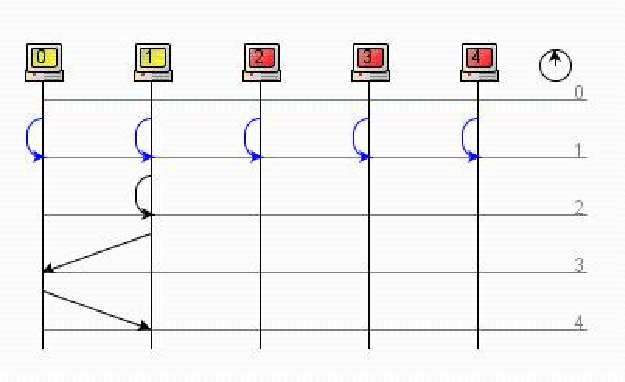
\includegraphics{images/p1ReadSeq.pdf}
	\caption{Bezeichnung der Abbildung}
	\label{a1}
\end{figure}

\begin{table} %[hbtp]
	\centering
		\begin{tabular}{l | l l l l}
		\textbf{Prozesse} & \textbf{Zeit} $\rightarrow$ \\
		\hline
			$P_{1}$ & $W(x)1$ \\
			$P_{2}$ & & $W(x)2$ \\
			$P_{3}$ & & $R(x)2$ & & $R(x)1$\\
			$P_{4}$ & & & $R(x)2$ & $R(x)1$\\
		\end{tabular}
	\caption{Bezeichnung der Tabelle}
	\label{t1}
\end{table}


\section{Mathematische Formel}\index{Formel}
Mathematische Formeln bzw. Formulierungen k�nnen sowohl im
laufenden Text (z.B. $y=x^2$) oder abgesetzt und zentriert im Text
erscheinen. Gleichungen sollten f�r Referenzierungen nummeriert
werden (siehe Formel \ref{gl-1}).
\begin{equation}
\label{gl-1}
e_{i}=\sum _{i=1}^{n}w_{i}x_{i}
\end{equation}

Entscheidungsformel:

\begin{equation}
\psi(t)=\left\{\begin{array}{ccc}
1 &  \qquad 0 <= t < \frac{1}{2} \\
-1 &  \qquad \frac{1}{2} <= t <1 \\
0 & \qquad sonst
\end{array} \right.
\end{equation}


Matrix:\index{Matrix}
\begin{equation}
A = \left(
\begin{array}{llll}
a_{11} & a_{12} & \ldots & a_{1n} \\
a_{21} & a_{22} & \ldots & a_{2n} \\
\vdots & \vdots & \ddots & \vdots \\
a_{n1} & a_{n2} & \ldots & a_{nn} \\
\end{array}
\right)
\end{equation}

Vektor:\index{Vektor} 

\begin{equation}
\overline{a} = \left(
\begin{array}{c}
a_{1}\\
a_{2}\\
\vdots\\
a_{n}\\
\end{array}
\right)
\end{equation}

\section{S�tze, Lemmas und Definitionen}\index{Satz}\index{Lemma}\index{Definition}

S�tze, Lemmas, Definitionen, Beweise,\index{Beweis} Beispiele\index{Beispiel} k�nnen in speziell daf�r vorgesehenen Umgebungen erstellt werden.

\begin{definition}(Optimierungsproblem)

Ein \emph{Optimierungsproblem} $\mathcal{P}$ ist festgelegt durch ein Tupel
$(I_\mathcal{P}, sol_\mathcal{P}, m_\mathcal{P}, goal)$ wobei gilt

\begin{enumerate}
\item $I_\mathcal{P}$ ist die Menge der Instanzen,
\item $sol_\mathcal{P} : I_\mathcal{P} \longmapsto \mathbb{P}(S_\mathcal{P})$ ist eine Funktion, die jeder Instanz $x \in I_\mathcal{P}$ eine Menge zul�ssiger L�sungen zuweist,
\item $m_\mathcal{P} : I_\mathcal{P} \times S_\mathcal{P} \longmapsto \mathbb{N}$ ist eine Funktion, die jedem Paar $(x,y(x))$ mit $x \in I_\mathcal{P}$ und $y(x) \in sol_\mathcal{P}(x)$ eine
Zahl $m_\mathcal{P}(x,y(x)) \in \mathbb{N}$ zuordnet (= Ma� f�r die L�sung $y(x)$ der Instanz $x$), und
\item $goal \in \{min,max\}$.
\end{enumerate}

\end{definition}

\begin{example} MINIMUM TRAVELING SALESMAN (MIN-TSP)
\begin{itemize}
\item $I_{MIN-TSP} =_{def}$ s.o., ebenso $S_{MIN-TSP}$
\item $sol_{MIN-TSP}(m,D) =_{def} S_{MIN-TSP} \cap \mathbb{N}^m$ 
\item $m_{MIN-TSP}((m,D),(c_1, \ldots , c_m)) =_{def} \sum_{i=1}^{m-1} D(c_i, c_{i+1}) + D(c_m,c_1)$ 
\item $goal_{MIN-TSP} =_{def} min$
\end{itemize}
\begin{flushright}
$\qed$
\end{flushright}
\end{example}

\begin{theorem} Sei $\mathcal{P}$ ein \textbf{NP}-hartes Optimierungsproblem.
Wenn $\mathcal{P} \in$ \textbf{PO}, dann ist \textbf{P} = \textbf{NP}.
\end{theorem}

\begin{proof} Um zu zeigen, dass \textbf{P} = \textbf{NP} gilt, gen�gt es
wegen Satz A.30 zu zeigen, dass ein einziges \textbf{NP}-vollst�ndiges
Problem in \textbf{P} liegt. Sei also $\mathcal{P}'$ ein beliebiges \textbf{NP}-vollst�ndiges Problem.

Weil $\mathcal{P}$ nach Voraussetzung \textbf{NP}-hart ist, gilt insbesondere
$\mathcal{P}' \leq_T \mathcal{P}_C$. Sei $R$ der zugeh�rige
Polynomialzeit-Algorithmus dieser Turing-Reduktion.
Weiter ist $\mathcal{P} \in$ \textbf{PO} vorausgesetzt, etwa verm�ge eines
Polynomialzeit-Algorithmus $A$. Aus den beiden
Polynomialzeit-Algorithmen $R$ und $A$ erh�lt man nun
leicht einen effizienten Algorithmus f�r $\mathcal{P}'$: Ersetzt man
in $R$ das Orakel durch $A$, ergibt dies insgesamt eine polynomielle
Laufzeit. 
%\begin{flushright}
$\qed$
% \end{flushright}
\end{proof}

\begin{lemma} Aus \textbf{PO} $=$ \textbf{NPO} folgt \textbf{P} $=$ \textbf{NP}.
\end{lemma}

\begin{proof} Es gen�gt zu zeigen, dass unter der angegeben
Voraussetzung KNAPSACK $\in$ \textbf{P} ist.

Nach Voraussetung ist MAXIMUM KNAPSACK $\in$ \textbf{PO},
d.h. die Berechnung von $m^*(x)$ f�r jede Instanz $x$ ist
in Polynomialzeit m�glich. Um KNAPSACK bei Eingabe
$(x,k)$ zu entscheiden, m�ssen wir nur noch $m^*(x) \geq k$
pr�fen. Ist das der Fall, geben wir $1$, sonst $0$ aus. Dies
bleibt insgesamt ein Polynomialzeit-Algorithmus. 
\begin{flushright}
$\qed$
\end{flushright}
\end{proof}

\section{Fu�noten}

In einer Fu�note k�nnen erg�nzende Informationen\footnote{Informationen die f�r die Arbeit zweitrangig sind, jedoch f�r den Leser interessant sein k�nnten.} angegeben werden. Au�erdem kann eine Fu�note auch Links enthalten. Wird in der Arbeit eine Software (zum Beispiel Java-API\footnote{\url{http://java.sun.com/}}) eingesetzt, so kann die Quelle, die diese Software zur Verf�gung stellt in der Fu�note angegeben werden.

\section{Literaturverweise}\index{Literatur}
Alle benutzte Literatur wird im Literaturverzeichnis angegeben\footnote{Dazu wird ein sogennanter bib-File, literatur.bib verwendet.}. Alle angegebene Literatur sollte mindestens einmal im Text referenziert werden\cite{Coulouris:02}.
\chapter{Beispiel-Kapitel}

In diesem KAPITEL wird beschrieben, warum es unterschiedliche Konsistenzmodelle\index{Konsistenzmodelle} gibt. Au�erdem werden die Unterschiede zwischen strengen Konsistenzmodellen\index{Linearisierbarkeit} (Linearisierbarkeit, sequentielle Konsistenz)\index{sequentiell!Konsistenz} und schwachen Konsistenzmodellen\index{Konsistenz!schwach} (schwache Konsistenz, Freigabekonsistenz)\index{Freigabekonsistenz} erl�utert. Es wird gekl�rt, was Strenge und Kosten (billig, teuer) in Zusammenhang mit Konsistenzmodellen bedeuten.

\section{Warum existieren unterschiedliche Konsistenzmodelle?}

Laut \cite{Malte:97} sind mit der\index{Replikation} Replikation von Daten immer zwei gegens�tzliche Ziele verbunden: die Erh�hung der\index{Verf�gbarkeit} Verf�gbarkeit und die Sicherung der\index{Konsistenz} Konsistenz der Daten. Die Form der Konsistenzsicherung bestimmt dabei, inwiefern das eine Kriterium erf�llt und das andere dementsprechend nicht erf�llt ist (Trade-off zwischen Verf�gbarkeit und der Konsistenz der Daten). Stark konsistente Daten sind stabil, das hei�t, falls mehrere Kopien der Daten existieren, d�rfen keine Abweichungen auftreten. Die Verf�gbarkeit der Daten ist hier jedoch stark eingeschr�nkt. Je schw�cher die Konsistenz wird, desto mehr Abweichungen k�nnen zwischen verschiedenen Kopien einer Datei auftreten, wobei die Konsistenz nur an bestimmten Synchronisationspunkten gew�hrleistet wird. Daf�r steigt aber die Verf�gbarkeit der Daten, weil sie sich leichter replizieren lassen.

Nach \cite{Mosberger:93} kann die Performanzsteigerung der schw�cheren Konsistenzmodelle wegen der Optimierung\index{Optimierung} (Pufferung, Code-Scheduling, Pipelines) 10-40 Prozent betragen. Wenn man bedenkt, dass mit der Nutzung der vorhandenen Synchronisierungsmechanismen schw�chere Konsistenzmodelle den Anforderungen der strengen Konsistenz gen�gen, stellt sich der h�here programmiertechnischer Aufwand bei der Implementierung der schw�cheren Konsistenzmodelle als ihr einziges Manko dar.

In \cite{Cheriton:85} ist beschrieben, wie man sich Formen von DSM vorstellen k�nnte, f�r die ein beachtliches Ma� an\index{Inkonsistenz} Inkonsistenz akzeptabel w�re. Beispielsweise k�nnte DSM verwendet werden, um die Auslastung von Computern in einem Netzwerk zu speichern, so dass Clients f�r die Ausf�hrung ihrer Applikationen die am wenigsten ausgelasteten Computer ausw�hlen k�nnen. Weil die Informationen dieser Art innerhalb k�rzester Zeit ungenau werden k�nnen (und durch die Verwendung der veralteten Daten keine gro�en Nachteile entstehen k�nnen), w�re es vergebliche M�he, sie st�ndig f�r alle Computer im System konsistent zu halten \cite{Coulouris:02}. Die meisten Applikationen stellen jedoch strengere Konsistenzanforderungen.

\section{Klassifizierung eines Konsistenzmodells}

Die zentrale Frage, die f�r die Klassifizierung\index{streng}\index{schwach} (streng oder schwach) eines Konsistenzmodells von Bedeutung ist \cite{Coulouris:02}: wenn ein Lesezugriff auf eine Speicherposition erfolgt, welche Werte von Schreibzugriffen auf diese Position sollen dann dem Lesevorgang bereitgestellt werden? Die Antwort f�r das schw�chste Konsistenzmodell lautet: von jedem Schreibvorgang, der vor dem Lesen erfolgt ist, oder in der "`nahen"' Zukunft, innerhalb des definierten Betrachtungsraums, erfolgten wird. Also irgendein Wert, der vor oder nach dem Lesen geschrieben wurde.

F�r das strengste Konsistenzmodell, Linearisierbarkeit (atomic consistency), stehen alle geschriebenen Werte allen Prozessoren sofort zur Verf�gung: eine Lese-Operation gibt den aktuellsten Wert zur�ck, der geschrieben wurde, bevor das Lesen stattfand. Diese Definition ist aber in zweierlei Hinsicht problematisch. Erstens treten weder Schreib- noch Lese-Operationen zu genau einem Zeitpunkt auf, deshalb ist die Bedeutung von "`aktuellsten"' nicht immer klar. Zweitens ist es nicht immer m�glich, genau festzustellen, ob ein Ereignis vor einem anderen stattgefunden hat, da es Begrenzungen daf�r gibt, wie genau Uhren in einem verteilten System synchronisiert werden k�nnen.

Nachfolgend werden einige Konsistenzmodelle absteigend nach ihrer Strenge vorgestellt. Zuvor m�ssen wir allerdings kl�ren, wie die Lese- und Schreibe-Operationen in dieser Ausarbeitung dargestellt werden.

Sei $x$ eine Speicherposition, dann k�nnen Instanzen dieser Operationen wie folgt ausgedr�ckt werden:
\begin{itemize}
	\item $R(x)a$ - eine Lese-Operation\index{Operation!Lese}, die den Wert $a$ von der Position $x$ liest.
	\item $W(x)b$ - eine Schreib-Operation\index{Operation!Schreib}, die den Wert $b$ an der Position $x$ speichert.
\end{itemize}

\section{Linearisierbarkeit\index{Linearisierbarkeit} (atomic consistency)}

Die Linearisierbarkeit im Zusammenhang mit DSM kann wie folgt definiert werden:
\begin{itemize}
	\item Die verzahnte Operationsabfolge findet so statt: wenn $R(x)a$ in der Folge vorkommt, dann ist die letzte Schreib-Operation, die vor ihr in der verzahnten Abfolge auftritt, $W(x)a$, oder es tritt keine Schreib-Operation vor ihr auf und $a$ ist der Anfangswert von $x$. Das bedeutet, dass eine Variable nur durch eine Schreib-Operation ge�ndert werden kann.
	\item Die Reihenfolge der Operationen in der Verzahnung ist konsistent zu den \underline{Echtzeiten}\index{Echtzeiten}, zu denen die Operationen bei der tats�chlichen Ausf�hrung aufgetreten sind.
\end{itemize}

Die Bedeutung dieser Definition kann an folgendem Beispiel (Tabelle \ref{tab:1}) nachvollzogen werden. Es sei angenommen, dass alle Werte mit $0$ vorinitialisiert sind.

\begin{table}
	\centering
		\begin{tabular}{l | l l l l}
			\textbf{Prozesse} & \textbf{Zeit} $\rightarrow$ & \\
			\hline
			$P_{1}$ & $W(x)1$ & & $W(y)2$ \\
			$P_{2}$ & & $R(x)1$ & & $R(y)2$ \\
		\end{tabular}
	\caption{Linearisierbarkeit ist erf�llt}
	\label{tab:1}
\end{table}

Hier sind beide Bedingungen erf�llt, da die Lese-Operationen den zuletzt geschriebenen Wert zur�ckliefern. Interessanter ist es, zu sehen, wann die Linearisierbarkeit verletzt ist.

\begin{table}
	\centering
		\begin{tabular}{l | l l l l}
		\textbf{Prozesse} & \textbf{Zeit} $\rightarrow$ \\
		\hline
		$P_{1}$ & $W(x)1$ & $W(x)2$ \\
		$P_{2}$ & & & \color{red} $R(x)0$ & \color{black} $R(x)2$ \\
		\end{tabular}
	\caption{Linearisierbarkeit ist verletzt, sequentielle Konsistenz ist erf�llt.}
	\label{tab:2}
\end{table}

In diesem Beispiel (Tabelle \ref{tab:2}) ist die Echtzeit-Anforderung verletzt, da der Prozess $P_{2}$ immer noch den alten Wert liest, obwohl er von Prozess $P_{1}$ bereits ge�ndert wurde. Diese Ausf�hrung w�re aber sequentiell konsistent (siehe kommender Abschnitt), da es eine Verzahnung der Operationen gibt, die diese Werte liefern k�nnte ($R(x)0$, $W(x)1$, $W(x)2$, $R(y)2$). W�rde man beide Lese-Operationen des 2. Prozesses vertauschen, wie in der Tabelle \ref{tab:3} dargestellt, so w�re keine sinnvolle Verzahnung mehr m�glich.

\begin{table}
	\centering
		\begin{tabular}{l | l l l l}
		\textbf{Prozesse} & \textbf{Zeit} $\rightarrow$ \\
		\hline
		$P_{1}$ & $W(x)1$ & $W(x)2$ \\
		$P_{2}$ & & & \color{red} $R(x)2$ &  \color{red} $R(x)0$ \\
			
		\end{tabular}
	\caption{Linearisierbarkeit und sequentielle Konsistenz sind verletzt.}
	\label{tab:3}
\end{table}

In diesem Beispiel sind beide Bedingungen verletzt. Selbst wenn die Echtzeit, zu der die Operationen stattgefunden haben, ignoriert wird, gibt es keine Verzahnung einzelner Operationen, die der Definition entsprechen w�rde.
\chapter{Zusammenfassung und Ausblick}

In diesem Kapitel soll die Arbeit noch einmal kurz zusammengefasst werden. Insbesondere sollen die wesentlichen Ergebnisse Ihrer Arbeit herausgehoben werden. Erfahrungen, die z.B. Benutzer mit der Mensch-Maschine-Schnittstelle gemacht haben oder Ergebnisse von Leistungsmessungen sollen an dieser Stelle pr�sentiert werden. Sie k�nnen in diesem Kapitel auch die Ergebnisse oder das Arbeitsumfeld Ihrer Arbeit kritisch bewerten. W�nschenswerte Erweiterungen sollen als Hinweise auf weiterf�hrende Arbeiten erw�hnt werden.
% ...
%--------------------------------------------------------------------------
\backmatter                        		% Anhang
%-------------------------------------------------------------------------
\bibliographystyle{geralpha}			% Literaturverzeichnis
\bibliography{literatur}     			% BibTeX-File literatur.bib
%--------------------------------------------------------------------------
\printindex 							% Index (optional)
%--------------------------------------------------------------------------
\begin{appendix}						% Anh�nge sind i.d.R. optional
   \chapter{Glossar}

\abbreviation{DisASTer}		{DisASTer (Distributed Algorithms Simulation Terrain), A platform for the Implementation of Distributed Algorithms}
\abbreviation{DSM}			{Distributed Shared Memory}
\abbreviation{AC}			{Linearisierbarkeit (atomic consistency)}
\abbreviation{SC}			{Sequentielle Konsistenz (sequential consistency)}
\abbreviation{WC}			{Schwache Konsistenz (weak consistency)}
\abbreviation{RC}			{Freigabekonsistenz (release consistency)}
			% Glossar   
\end{appendix}

\end{document}
